%\documentstyle[epsf,twocolumn]{jarticle}       %LaTeX2.09仕様
\documentclass{jarticle}     %pLaTeX2e仕様

%\usepackage[backend=bibtex, style=numeric]{biblatex}
%\addbibresource{sankou.bib}
%%%%%%%%%%%%%%%%%%%%%%%%%%%%%%%%%%%%%%%%%%%%%%%%%%%%%%%%%%%%%%
%%
%%  基本 バージョン
%%
%%%%%%%%%%%%%%%%%%%%%%%%%%%%%%%%%%%%%%%%%%%%%%%%%%%%%%%%%%%%%%%%
\setlength{\topmargin}{-45pt}
%\setlength{\oddsidemargin}{0cm}
\setlength{\oddsidemargin}{-7.5mm}
%\setlength{\evensidemargin}{0cm}
\setlength{\textheight}{24.1cm}
%setlength{\textheight}{25cm}
\setlength{\textwidth}{17.4cm}
%\setlength{\textwidth}{172mm}
\setlength{\columnsep}{11mm}

\setlength{\intextsep}{8pt}
\setlength{\textfloatsep}{8pt}
\setlength{\floatsep}{1pt}

\kanjiskip=.07zw plus.5pt minus.5pt



%【節がかわるごとに(1.1)(1.2) …(2.1)(2.2)と数式番号をつけるとき】
%\makeatletter
%\renewcommand{\theequation}{%
%\thesection.\arabic{equation}} %\@addtoreset{equation}{section}
%\makeatother

%\renewcommand{\arraystretch}{0.95} 行間の設定

\usepackage[dvipdfmx]{graphicx}   %pLaTeX2e仕様(\documentstyle ->\documentclass)
\usepackage{scalefnt}
\usepackage{bm}
\usepackage{here}
\usepackage{url}
\usepackage{amsmath}
\usepackage{amsfonts}
\usepackage[subrefformat=parens]{subcaption}
\captionsetup{compatibility=false}
%%%%%%%%%%%%%%%%%%%%%%%%%%%%%%%%%%%%%%%%%%%%%%%%%%%%%%%%
\usepackage{comment}
\usepackage{subcaption}
\usepackage{multirow}
\usepackage{nidanfloat}
\usepackage[dvipdfmx]{hyperref}

\usepackage[normalem]{ulem}
\useunder{\uline}{\ul}{}

\begin{document}

\twocolumn[
\noindent
\hspace{1em}

令和2年10月20日(水) ゼミ資料
\hfill
\ \ B4 高山 裕成

\vspace{2mm}
\hrule
\begin{center}
{\Large  進捗報告}
\end{center}
\hrule
\vspace{3mm}
]


% \footnotesize

\section{今週あったこと}
\begin{itemize}
  \item i2v の PyTorch 移植完了
  \item データセット引継ぎとアノテーション作業
  \item データセットの再構築
\end{itemize}

\section{i2v の PyTorch 移植完了}
\begin{itemize}
  \item 結局, 自分でラッパーを書いて動作確認をした
  \item .caffemodel を .npz にしてから .pth にした
\end{itemize}

図 \ref{fig:miku} に, 自作ラッパー版とオリジナルの出力比較を載せる. 入力はオリジナルの GitHub でも紹介されているデモ用画像を用い, 確率のしきい値は 0.5 とした. 図 \ref{fig:miku} より, おおよその結果は一致したが所々出力が異なった. また, 4096 次元の分散表現同士のコサイン類似度は 0.979 であった. なぜ違いが生まれるのかについては要検証だが, ファインチューニングもできるようになった.

\begin{figure*}[!bth]
  \begin{center}
    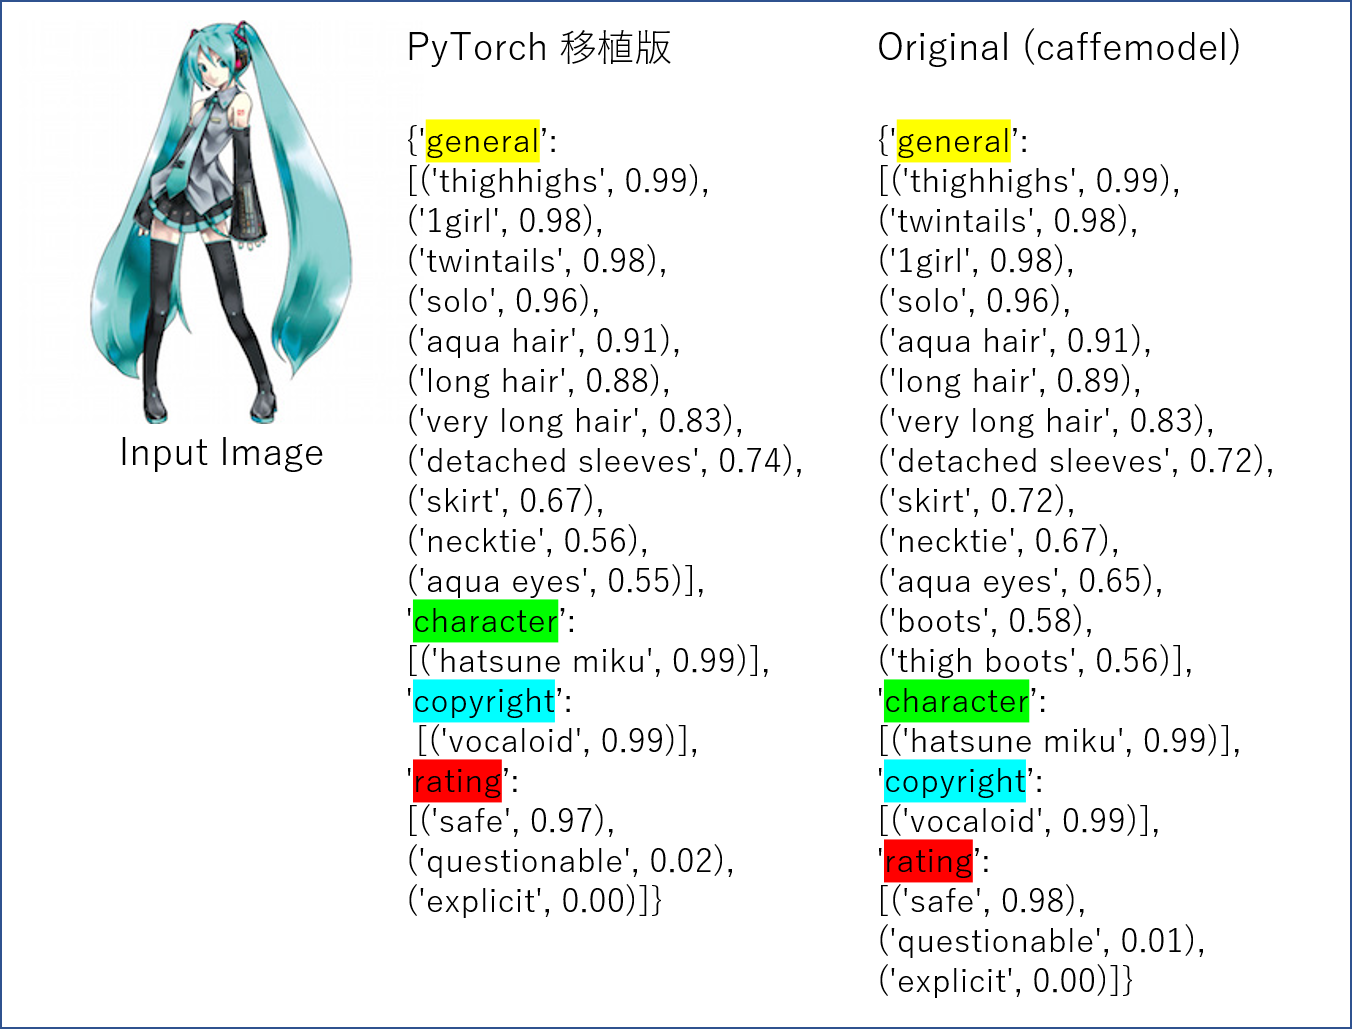
\includegraphics[scale=0.4]{miku.png}
    \caption{i2v 比較} %タイトルをつける
    \label{fig:miku} %ラベルをつけ図の参照を可能にする
  \end{center}
\end{figure*}

\section{データセット引継ぎとアノテーション作業}
寺内さんから改めて 4 コマ漫画ストーリーデータセット のオリジナルと, 寺内さんが用意してくれた各コマについてレイヤー分けされたものと結合するスクリプトを頂いた. これを利用することでほとんどのデータについてはセリフの白抜きだけでなく任意のレイヤー結合が可能. ごく一部のデータは全レイヤーが結合された状態のものしかないので手作業で切らなければならないという現状. 後世のためにもアノテート作業(レイヤー分けされたものがどの種類か, という作業)を完成しておいた方が良い.

\section{データセットの再構築}
先週示したデータ不備をもとに再構築中です.

\section{usagi}
一応, cuda が機能するようになっていたが遅い気がする?

\end{document}
